\subsection{两个平面的位置关系}\label{subsec:1-12}

图 \ref{fig:ltjh-1-37} 是一座高层建筑,它的正面和背面无论怎样延展都不会相交,也就是,它的正面和背面没有公共点;
它的正面和侧面则有一条公共直线。这些面的位置关系,反映出两个不重合的平面的不同位置关系。

如果两个平面没有公共点,我们说这\zhongdian{两个平面互相平行}。

\begin{figure}[htbp]
    \centering
    \begin{minipage}[b]{7cm}
        \centering
        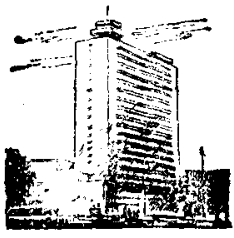
\includegraphics[width=4cm]{../pic/ltjh-ch1-37.png}
        \caption{}\label{fig:ltjh-1-37}
    \end{minipage}
    \qquad
    \begin{minipage}[b]{7cm}
        \centering
        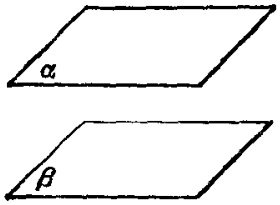
\includegraphics[width=4cm]{../pic/ltjh-ch1-38.png}
        \caption{}\label{fig:ltjh-1-38}
    \end{minipage}
\end{figure}


两个平面的位置关系只有:

(1)\zhongdian{两平面平行} —— 没有公共点;

(2)\zhongdian{两平面相交} —— 有一条公共直线。

画两个互相平行的平面时,要注意使表示平面的两个平行四边形的对应边平行(图 \ref{fig:ltjh-1-38})。

平面 $\alpha$ 与 $\beta$ 平行,记作 $\alpha \pingxing \beta$。


\begin{lianxi}

\xiaoti{举出两个平面平行和相交的一些实例。}

\xiaoti{画两个平行平面和分别在这两个平面内的两条平行直线,再画一个经过这两条平行直线的平面。}

\end{lianxi}
